\subsection{Sprint 1}

\subsubsection{Sprint start}

Sprint 1 was the first actual sprint that the team had. The goals that were set for the sprint was to get a meeting with the customer,
get a better grip of what the tasks ahead was, continuous research about the task and set all the team members roles.

\subsubsection{Sprint burndown}

The sprint burndown chart, the blue line represents the projected burndown of the project. It is calculated so that total points are divided by the number of days left in the sprint. The red line represents the story points that actually was completed and is calculated by subtracting the total story points by actual accepted story points.

Very little progress was made in the sprint burndown chart for the first sprint, shown in figure~\ref{fig:sprint1burndown}. This was mainly caused by the team's improper use of Yodiz.

\begin{figure}[H]
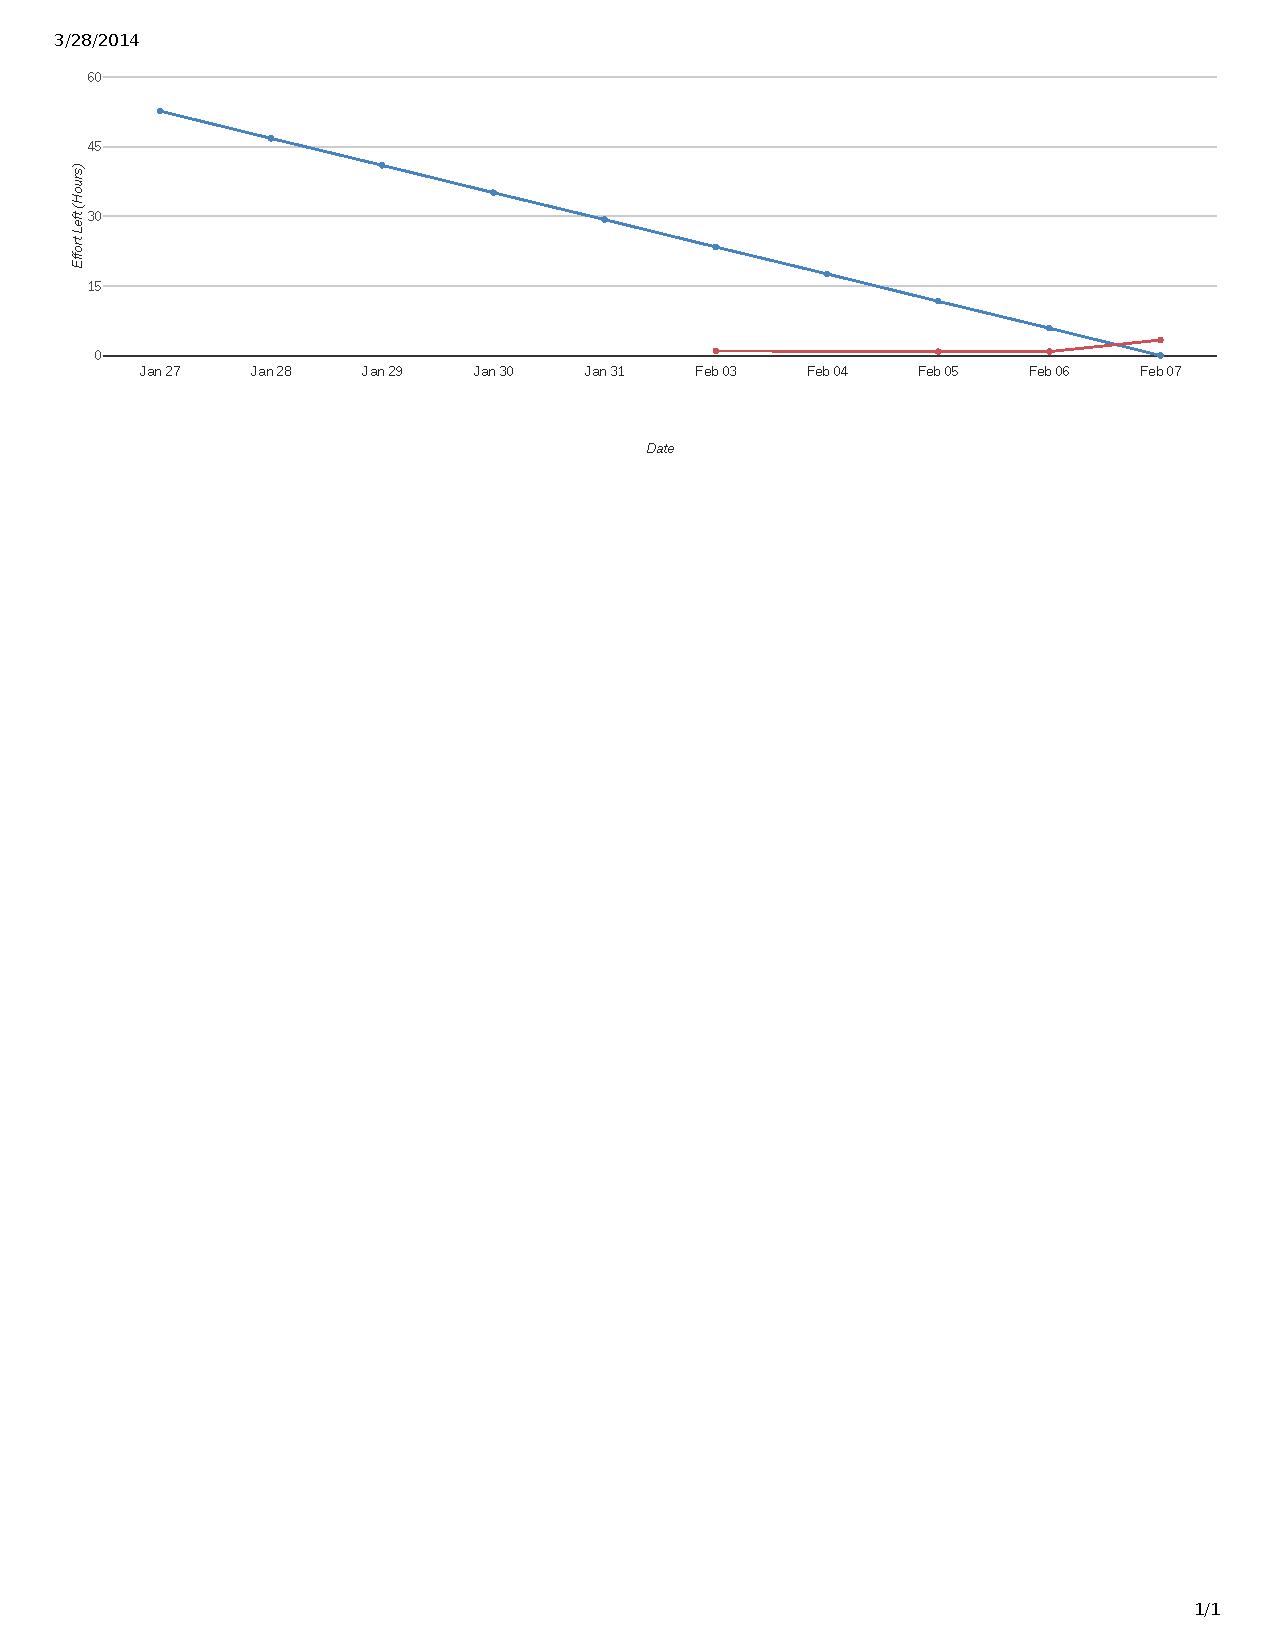
\includegraphics[width=\textwidth, trim= 1cm 21cm 1cm 1cm, clip=true]{ch/devProcess/fig/burndown1.pdf}
\caption{Sprint 1 burndown chart}
\label{fig:sprint1burndown}
\end{figure}

\subsubsection{Sprint backlog}

The backlog and time usage result.

\begin{table}[H]
		\begin{tabular}{|l|p{7cm}|p{2.2cm}|p{1.5cm}|p{1.5cm}|}%
    \hline \bfseries User story & \bfseries Details & \bfseries Hours \newline estimated & \bfseries Hours spent & \bfseries Hours left
    \csvreader[head to column names]{ch/devProcess/sprint1/userstories.csv}{}% use head of csv as column names
    {\\\hline \id & \title & \estimated & \spent & \left}\\\hline% specify your coloumns here
    %\hline
    \end{tabular}
	\caption{Sprint 1 backlog}
\end{table}

\subsubsection{Sprint end}
The main focus of this sprint was the project management part. The scrum model was chosen as project methodology. 
A rough project plan was made, and concepts for the application was made.
The customer was very pleased with the teams ideas and concepts for the app, and approved of the temporary specification. 
The team began writing documentation in \LaTeX. To uphold the scrum model, the tool Yodiz was chosen. More about Yodiz can be found in section~\ref{sec:yodiz}.

The customer wanted the application to be developed at the Android platform. Android-studio became the tool of choice for this.

The team members deemed sprint 1 very successful.

